\documentclass{article}
\usepackage{amsmath,graphicx}
\title{Sparse Signals Improve Accuracy Under a Fixed Research Budget}
\author{Synthetic Research Fixture}
\begin{document}
\begin{abstract}
This synthetic study tests whether selecting informative observations improves accuracy under a fixed annotation budget. We compare a sparse-signal method with a uniform baseline on two datasets. The reported scope is restricted to the evaluated datasets.
\end{abstract}
\section{Research question}
Can informative observations improve prediction accuracy without increasing the annotation budget? Uniform sampling spends part of the budget on redundant observations.
\section{Prior work and gap}
Prior sampling approaches prioritize coverage. They do not directly optimize the information retained under the same fixed budget. This study evaluates that gap without claiming a universal improvement.
\section{Method}
The method ranks observations by uncertainty and selects a diverse subset. The baseline uses the same model and the same annotation budget. We repeat each experiment with five random seeds.
\begin{equation}
S = \frac{1}{n}\sum_{i=1}^{n} u_i
\label{eq:score}
\end{equation}
\section{Results}
On the first dataset, accuracy is 87.1\% for the proposed method and 80.2\% for the baseline. The measured gain is 6.9 percentage points under the same budget. On the second dataset, the improvement is smaller and depends on the selected subset.
\begin{figure}
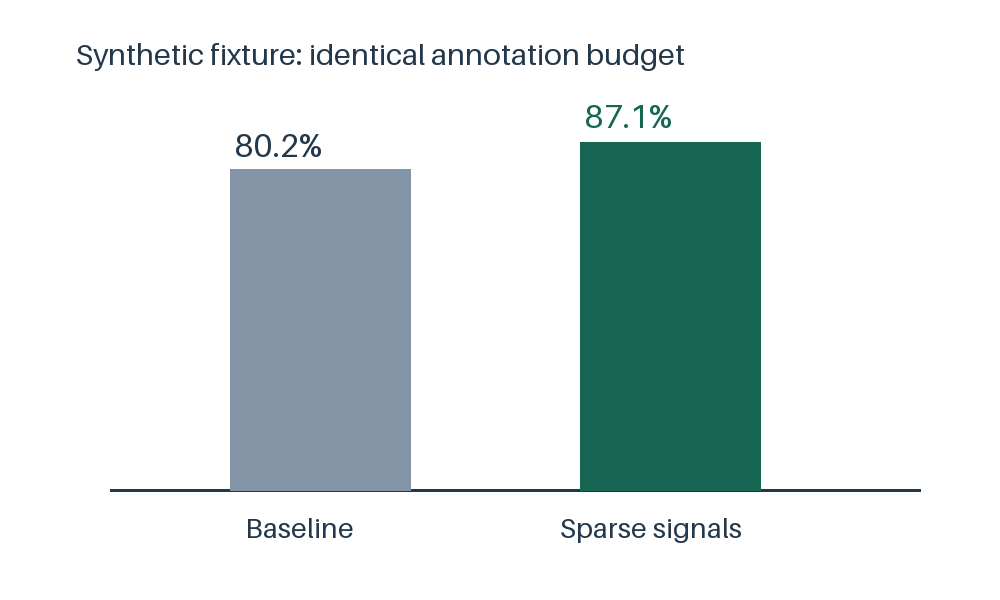
\includegraphics[width=.8\linewidth]{accuracy.png}
\caption{\textbf{Measured accuracy} on the first dataset under an identical annotation budget: baseline 80.2\%, proposed method 87.1\%. Error bars are not available in this synthetic fixture.}
\label{fig:accuracy}
\end{figure}
\section{Ablation}
Removing diversity selection lowers first-dataset accuracy to 84.0\%. This supports the contribution of the selection step in the evaluated setting. It does not isolate every possible interaction between model and data.
\begin{table}
\caption{First-dataset accuracy under the same annotation budget.}
\begin{tabular}{lr}
Method & Accuracy \\
Uniform baseline & 80.2\% \\
Without diversity & 84.0\% \\
Sparse signals & 87.1\% \\
\end{tabular}
\end{table}
\section{Limitations}
The evaluation covers only two datasets and five seeds. The study does not establish performance in new domains. Annotation quality and fairness across subgroups were not evaluated.
\section{Conclusion}
Sparse informative observations improve first-dataset accuracy under a fixed budget. The next step is to evaluate transfer to new domains before making broader claims.
\end{document}
